\section{Experiment}
To verify the reliability of the water balance model for high-power fuel cell systems, it is necessary to record the water-containing state of the high-power fuel cell system when it reaches water balance under different operating conditions. Therefore, the experimental conditions should meet the following three points:
% 为了验证高功率燃料电池系统水平衡模型的可靠性,需要记录高功率燃料电池系统在不同工况下达到水平衡时的含水状态。 因此,实验条件应满足以下三点:
\begin{itemize}
	\item The selected operating parameters within normal operating range of the fuel cell system, reducing effects by faults in FC(Fuel Cell) system other than water content faults (gas supply insufficiency, air compressor surge, proportional valve failure, etc.)
	      % 所选运行参数应在燃料电池系统正常运行范围内,避免燃料电池系统出现含水故障以外的其他故障(如反应气体供应不足、空压机喘振、比例阀故障等)。
	\item By designing experiments that manifest more pronounced phenomena under both dry and flooded conditions, the study would investigates the effects of water content faults in fuel cell systems.
	      % 为了研究燃料电池系统出现含水故障时的现象,设计的实验需要反映干燥和淹水条件下更明显的现象
	\item The steady-state operation time should be long enough to ensure that the water content inside the fuel cell is in dynamic balance during this period, avoiding the impact of dynamic characteristics on the experimental results.
	      % 稳态运行时间应足够长,以保证在此期间燃料电池内部的含水量处于动态平衡,避免动态特性对实验结果的影响。
\end{itemize}
\subsection{Experiment Design}
Literature review highlights that the air-to-fuel ratio, operating temperature, and load current are the predominant factors affecting water content within the fuel cell\cite{legrosFirstResultsPEMFC2011}. Given the temperature inside stack can not be measured during operation, the inlet temperature of coolant is treated as working temperature in this research, and the working temperature in the following text refers to the inlet temperature of the coolant. According to the operating conditions recommended by the system side, a three-factor five-level water content experiment was designed. The parameters of the experiment are shown in Table \ref{tab:WaterStateExperimentalParameterTable}.
% 文献表明,对燃料电池内部含水量影响最大的因素是空气计量比、工作温度和负载电流\cite{legrosFirstResultsPEMFC2011}。由于运行时无法测量电堆内部温度,因此本文采用冷却剂入口温度作为工作温度,下文中的工作温度均指冷却剂入口温度。根据系统方推荐的运行工况,设计了三因素五级含水量实验。实验的参数显示在\ref{tab:WaterStateExperimentalParameterTable}中。
\begin{table}
	\centering

	\begin{center}
		\caption{Water state experimental parameter table}
		\label{tab:WaterStateExperimentalParameterTable}
		\begin{tabular}{ccc}
			% \hline
			\toprule
			\textbf{\makecell{Load current(A) /          \\currency density(A·cm\raise0.5ex\hbox{-2})}}   & \textbf{Working temperature(\textdegree C)} & \textbf{Air metering ratio} \\
			% \hline
			\midrule
			120/0.4 & 55,60,65,70,73 & 2,2.2,2.4,2.6,2.8 \\
			210/0.7 & 55,60,65,70,73 & 1.8,2,2.2,2.4     \\
			300/1.0 & 63,65,68,70,73 & 1.8,2,2.2,2.4     \\
			% \hline
			\bottomrule
		\end{tabular}
	\end{center}

\end{table}

Literatures\cite{wuDiagnosticToolsPEM2008} indicates that the time required for the fuel cell system to reach water balance is generally a few seconds to ten minutes. Therefore, each test point ran for 20 minutes, and it was assumed that the fuel cell was in the process of establishing water balance within the first 15 minutes, and no data was recorded for this process, and the data obtained in the last 5 minutes was recorded. During the test, if a single cell voltage is too low or other faults cause the fuel cell system to shut down, the data of this operating point will be removed.
% 文献\cite{wuDiagnosticToolsPEM2008}表明,燃料电池系统达到水平衡所需的时间一般为几秒到十分钟。因此,每个测试点运行 20 分钟,并假设燃料电池在前 15 分钟内处于建立水平衡的过程,并且该过程没有记录数据,最后 5 分钟获得的数据 被记录。测试过程中,如果单节电池电压过低或其他故障导致燃料电池系统关闭,则该工作点的数据将被清除。

% 2.2 章
\subsection{Test platform introduction}
The high-power fuel cell system used in this article is shown in Fig \ref{fig:PowerSystemDiagram}, manufactured by AT\&M Environmental Engineering Technology Co. With rated net output power of 100kW, the stack is composed of 410 single cells. High-pressure dry hydrogen gas enters the anode of the reaction stack after being depressurized by the solenoid valve and proportional valve. The liquid water in the residual hydrogen is separated by the gas-water separation device and intermittently discharged through the drain valve.
% 本文采用的大功率燃料电池系统如图 2 所示,由 AT&M 环境工程技术有限公司生产。该燃料电池系统的额定净输出功率为 100kW,电堆由 410 块单电池组成。高压干燥氢气经电磁阀和比例阀减压后进入反应堆阳极。残余氢气中的液态水被气水分离装置分离,并通过排水阀间歇排放。
\begin{figure}[h]
	\centering

	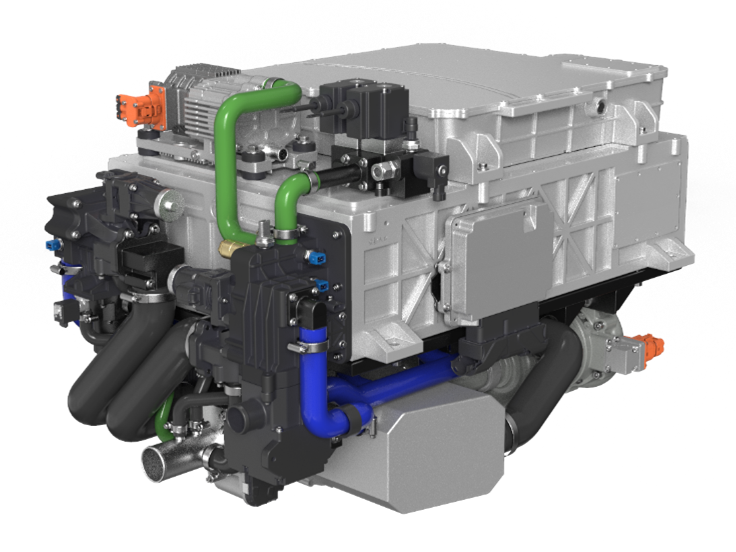
\includegraphics[scale=0.4]{Research_pictures/picture2.png}
	\caption[short]{power system diagram}
	\label{fig:PowerSystemDiagram}
\end{figure}

For the above fuel cell system, the water balance model can be represented as
% 对于上述燃料电池系统,水平衡模型可表示为
\begin{equation} \label{waterBalanceModel}
	\frac{d m_{w,s y s}}{d t}=Q_{v,i n,s y s}+Q_{w,g e n,c a}-Q_{w,o u t,c a}-Q_{w,o u t,a n}
\end{equation}

In Formula (\ref{waterBalanceModel}), epresents the water
\begin{itemize}
	\item $m_(w,sys)$ represents the water content inside the fuel cell system, in grams; %代表燃料电池系统内的水含量,以克为单位。
	\item $Q_(v,in,sys)$ represents the flow rate of water vapor entering the fuel cell system, in g/s; %表示进入燃料电池系统的水蒸气的流量,单位为 g/s
	\item $Q_(w,gen)$ represents the water flow generated by the electrochemical reaction, in g/s; %表示电化学反应产生的水流量,单位为 g/s
	\item $Q_(w,out,ca)$ represents the water flow out of the system from the air subsystem, in g/s; %表示从空气子系统流出系统的水流量,单位为 g/s;
	\item $Q_(w,out,an)$ represents the water flow out of the system from the hydrogen subsystem, in g/s; %表示从氢气子系统流出系统的水流量,单位为 g/s
\end{itemize}
Taking the fuel cell system during steady-state operation as the research object, the change in the water content of the auxiliary system of the fuel cell system can be ignored, that is,
% 以稳态运行时的燃料电池系统为研究对象,燃料电池系统辅助系统含水量的变化可以忽略不计,即
\begin{equation}\label{changeInWaterContent}
	\frac{d m_{w,s t k}}{d t}=\frac{d m_{w,s y s}}{d t}
\end{equation}
Each part of the equation required for the water balance model is described below:
\subsubsection{Water flow into the system}
Since the hydrogen entering the system is high-pressure hydrogen with a purity of 99.99\%, water vapor mainly enters the system with the air. By recording the temperature, humidity, pressure of the environment during the reaction process, and the air flow entering the system, the water flow entering the system can be calculated.
% 由于进入系统的氢气是纯度为 99.99% 的高压氢气,因此水蒸气主要随空气进入系统。通过记录反应过程中环境的温度、湿度、压力以及进入系统的空气流量,可以计算出进入系统的水流量。
\begin{equation}\label{waterFlowEnteringSystemCalculation}
	Q_{v,i n,s y s}={\frac{Q_{a i r;i n,s y s}\cdot P_{v a m b} \cdot M_{v}}{M_{a} \cdot P_{a m b}}}={\frac{Q_{a i r;i n,s y s}\cdot (P_{a m b} - P_{s a t} \ast RH)\cdot M_{v}}{M_{a} \cdot P_{a m b}}}
\end{equation}
In Formula(\ref{waterFlowEnteringSystemCalculation}),
\begin{itemize}
	\item $Q_{a i r;i n,s y s}$ stands for air flow into the system, in g/s;
	\item $P_{a m b}$ stands for environmental pressure, in kPa;
	\item $R_{v}$ represents the relative humidity of the environment;
	\item $P_{sat}$ represents the saturated vapor pressure of the environment, which can be calculated using the saturated water vapor pressure formula.
\end{itemize}

\begin{equation}
	p_{sat}\,= \exp \left(9.3876-{\frac{3826.36}{T_{a m b}-45.47}}\right)\times\,10^{3}
\end{equation}
\begin{itemize}
	\item $T_{amb}$ represents environmental temperature, K;
	\item $M_{v}$ represents water relative molecule mass, in g/mol;
	\item $M_{a}$ represents water relative molecule mass, in g/mol;
\end{itemize}
\subsection*{Water flow by electrochemical reaction}
The water flow produced by electrochemical reaction can be presented as formula below:
\begin{equation}
	Q_{v,g e n,c a}=\frac{{N\cdot M_{v}\cdot I_{s t}}}{2F}
\end{equation}
\begin{itemize}
	\item $N$ represents the number of single cells in the fuel cell stack.
	\item $I_{st}$ represents load current, in A.
	\item $F$ stands for faraday constant, which is 96485C/mol.
\end{itemize}
\subsubsection{The water flow out of the system from the air side and the hydrogen side}
To measure the water flow out of the system from the air and hydrogen sides, this article has designed an exhaust water content detection device centered on condensation.
% 为了测量从空气侧和氢气侧流出系统的水流量,本文设计了一种以冷凝为核心的排气含水量检测装置。
\begin{figure}
	\centering

	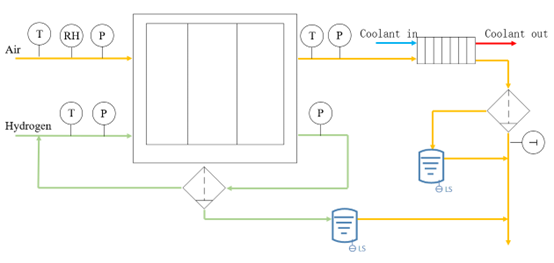
\includegraphics[scale=0.6]{Research_pictures/picture3.png}
	\caption[short]{Schematic diagram of exhaust gas water content detection device}
	\label{fig:water_detection_device_diagram}
\end{figure}
The exhaust water content detection device on the air side is composed of a heat exchanger, a water separator, a temperature sensor, and a water collection device with a liquid level sensor. The basic principle is to condense the high-temperature supersaturated exhaust gas on the air side, and then separate the liquid water inside from the exhaust gas through the water separator, thus obtaining saturated low-temperature exhaust gas and liquid water. Collect the separated liquid water and collect the liquid level with a liquid level sensor.
% 空气侧排气含水量检测装置由热交换器、水分离器、温度传感器和带有液位传感器的集水装置组成。 其基本原理是将高温过饱和废气在空气侧冷凝,然后通过水分离器将内部的液态水与废气分离,从而获得饱和低温废气和液态水。 收集分离出的液态水,并用液位传感器采集液位。
Therefore, the water flow out of the system from the air side is composed of two parts: the liquid water collected in the air side collection device and the water vapor carried in the saturated steam after water vapor separation, that is,
% 因此,从空气侧流出系统的水由两部分组成:空气侧收集装置收集的液态水和水蒸气分离后的饱和蒸汽中携带的水蒸气,即
\begin{equation}
	\label{waterFlowOutOfTheSystem}
	Q_{w,out,ca}={\frac{d m_{w,cacollect}}{d t}}+{\frac{Q_{air,out,sys} \cdot p_{v,sat}\cdot M_{v}}{M_{a} \cdot P_{a m b}}}
\end{equation}
In Formula(\ref{waterFlowOutOfTheSystem}),
\begin{itemize}
	\item $m_{w,cacollect}$ represents the mass of the liquid collected by the exhaust water collection device on the air side, in grams(g);
	\item $Q_{air,out,sys}$ represents the air flow out of the system, in g(gram)/s(second), which can be calculated by the following formula.
\end{itemize}
The $Q_{air,out,sys}$ is represented as below:
\begin{equation}
	\label{airFlowOutOfTheSystem}
	Q_{air,outsys}=Q_{air,in,sys}-Q_{o,recat,ca}+Q_{v,gen,ca}-{\frac{dm_{w,cacolect}}{dt}}
\end{equation}
Since the hydrogen return circuit of the system is equipped with a water separator, the water content detection device on the hydrogen side mainly collects liquid water and a small amount of hydrogen, with less gaseous water, which does not significantly affect the experimental results. Therefore, the exhaust water content detection device on the hydrogen side only has a water collection device with a liquid level sensor, which is used to record the water flow discharged from the hydrogen side.
% 由于系统氢气回流回路设有水分离器,氢气侧水分检测装置主要收集液态水和少量氢气,气态水较少,对实验结果没有明显影响。 因此氢气侧排气含水量检测装置只有一个带有液位传感器的集水装置,用于记录氢气侧排出的水流量。
\begin{equation}
	Q_{w,out,an}={\frac{dm_{w,ancollect}}{dt}}
\end{equation}
$m_{w,ancollect}$ represents the mass of the liquid collected by the exhaust water collection device on the hydrogen side, in grams(g).

\subsubsection{Test methods}
In sequence, turn on host computer, system controller, electronic load, auxiliary devices, and impedance testing system; Turn on the water pump, solenoid valve, proportional valve, back pressure valve, air compressor, drain valve, and hydrogen circulation pump in sequence, setting the anode inlet gas pressure 10kPa higher than the cathode inlet gas pressure ($\Delta p=20kPa$).
% 依次打开主机、系统控制器、电子负载、辅助设备、阻抗测试系统; 依次打开水泵、电磁阀、比例阀、背压阀、空压机、排水阀、氢气循环泵,设置阳极入口气体压力比阴极入口气体压力高10kPa($\Delta p=20kPa $)。
\par
Gradually load the system to 120A, adjust the speed of the air compressor and the opening angle of the back pressure valve, so that the air flow rate reaches the air metering coefficient of 2.8 corresponding to the target current, gradually raise the working temperature to $55\pm1^{\circ}C$, and start the temperature closed-loop control program to maintain this temperature; After the working temperature is stable at $55\pm1^{\circ}C$, start timing and run for a total of 15 minutes; Adjust the speed of the air compressor and the opening angle of the back pressure valve, so that the air metering ratio gradually decreases in the range of $2 \sim 2.8$ with a step size of 0.2; Raise the working temperature to $60\pm1^{\circ}C$, $65\pm1^{\circ}C$, $70\pm1^{\circ}C$ , $73\pm1^{\circ}C$, repeat the testing phase and record the experimental data.
% 逐渐将系统加载至120A,调节空压机的转速和背压阀的开启角度,使空气流量达到目标电流对应的空气计量系数2.8,逐渐将工作温度升至$55 \pm1^{\circ}C$,并启动温度闭环控制程序,维持该温度; 工作温度稳定在$55\pm1^{\circ}C$后,开始计时,共运行15分钟; 调节空压机转速和背压阀开启角度,使空气计量比在2~2.8范围内逐渐减小,步长为0.2; 将工作温度升高至$60\pm1^{\circ}C$、$65\pm1^{\circ}C$、$70\pm1^{\circ}C$、$73\pm1^{\circ}C$,重复 测试阶段并记录实验数据。
\par
Load up to 210A, 300A, repeat all recording steps, until all operating points water content detection experiments are completed.
% 加载至210A、300A,重复所有记录步骤,直至所有工作点含水量检测实验完成。
\par
Gradually reduce the load to 0A, purging circuit with nitrogen, turn off the machine, and power down in sequence.
% 逐渐将负载降至0A,用氮气吹扫电路,关闭机器,依次断电。